\documentclass{tufte-handout}
\usepackage{amsmath}
\usepackage[utf8]{inputenc}
\usepackage{mathpazo}
\usepackage{booktabs}
\usepackage{microtype}

\usepackage{tikz}

\pagestyle{empty}


\title{Word Ladders Report}
\author{Dennis Sadeler Shapira and Jonas Lomholdt}

\begin{document}
  \maketitle

  \section{Results}

  The following table summarizes our results:

  \bigskip\noindent
  \begin{tabular}{lr}
    \toprule
    Input file & MST total weight \\ \midrule
    USA-highway-miles.txt	 & 16598 \\
    tinyEWG-alpha.txt & 183 \\ \bottomrule
  \end{tabular}

  \bigskip
  The MST we found in tinyEWG-alpha.txt can be drawn like this:

  \medskip
  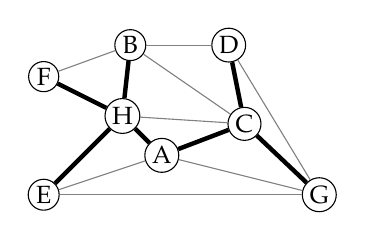
\begin{tikzpicture}[
      scale = .5,
      every node/.style = {
        circle, draw, black, inner sep = 1pt, font = \small},
      every path/.style = {gray}
      ]
    \node (A) at (3,1) {A}; % 0
    \node (B) at (2.2,3.8) {B}; % 1
    \node (C) at (5.1,1.8) {C}; % 2
    \node (D) at (4.7,3.8) {D}; % 3
    \node (E) at (0,0) {E}; % 4
    \node (F) at (0,3) {F}; % 5
    \node (G) at (7,0) {G}; % 6
    \node (H) at (2,2) {H}; % 7
    
    \draw (F)--(H);
    \draw (E)--(H);
    \draw (G)--(E);
    \draw (D)--(G);
    \draw (C)--(D);
    \draw (C)--(H);
    \draw (G)--(C);
    \draw (B)--(F);
    \draw (B)--(H);
    \draw (B)--(C);
    \draw (B)--(D);
    \draw (A)--(H);
    \draw (A)--(E);
    \draw (A)--(C);
    \draw (G)--(A);
    
    
    
   
    \begin{scope}[every path/.style={ultra thick}]
        \draw (A)--(H);
        \draw (C)--(D);
        \draw (B)--(H);
        \draw (A)--(C);
        \draw (F)--(H);
        \draw (E)--(H);
        \draw (G)--(C);
    \end{scope}
  \end{tikzpicture}
  
  


 2-7 34.00000  1-2 36.00000  0-2 26.00000  2-3 17.00000  
3: 3-6 52.00000  1-3 29.00000  2-3 17.00000  
4: 6-4 93.00000  0-4 38.00000  4-7 37.00000  
5: 1-5 32.00000  5-7 28.00000  
6: 6-4 93.00000  6-0 58.00000  3-6 52.00000  6-2 40.00000  
7: 2-7 34.00000  1-7 19.00000  0-7 16.00000  5-7 28.00000  4-7 37.00000 


  \section{Implementation details}

  We implemented the algorithm of [$\ldots$], using [$\ldots$].%
  \sidenote{%
    Explain what you did.
    Prim?
    Kruskal?
    Which priority queue?
    How did you check connectivity?
    Be very brief.
    Three sentences are a lot.}
  The total running time for implementation is $O(n^3+\log^2 m)$.\sidenote{%
  Replace as necessary.
  Use $n$ for the number of vertices,
    $m$ for the number of edges in the input graph.}
    
    We implemented the algorithm of Prim using the first-in-first-out (FIFO) priority queue. In order to check connectivity we assign a boolean to each vertex to keep track whether the vertex has yet been visited or not.

\end{document}
